% This is a placeholder file for a NeurIPS 2025 submission.
% Use this as a starting point to write your paper.
%
% To compile:
% 1. Make sure you have the neurips_2025.sty file in the same directory.
% 2. Make sure you have your references.bib file in the same directory.
% 3. Run pdflatex on this file. For example:
%    pdflatex my_neurips_paper.tex
%    bibtex my_neurips_paper
%    pdflatex my_neurips_paper.tex
%    pdflatex my_neurips_paper.tex
%
% For initial submission, DO NOT USE [preprint] or [final] options.
% The default ensures anonymity and adds line numbers for reviewers.

\documentclass{article}

% Recommended, but not required packages for NeurIPS 2025
\usepackage{neurips_2025}

% if you need to pass options to natbib, use, e.g.:
%     \PassOptionsToPackage{numbers, compress}{natbib}
% before loading neurips_2025
% \usepackage[numbers, compress]{natbib} % Example with natbib options



% to compile a preprint version, e.g., for submission to arXiv, add add the
% [preprint] option:
%     \usepackage[preprint]{neurips_2025}


% to compile a camera-ready version, add the [final] option, e.g.:
%     \usepackage[final]{neurips_2025}


% to avoid loading the natbib package, add option nonatbib:
%    \usepackage[nonatbib]{neurips_2025}


\usepackage[utf8]{inputenc} % allow utf-8 input
\usepackage[T1]{fontenc}    % use 8-bit T1 fonts
\usepackage{hyperref}       % hyperlinks
\usepackage{url}            % simple URL typesetting
\usepackage{booktabs}       % professional-quality tables
\usepackage{amsfonts}       % blackboard math symbols
\usepackage{nicefrac}       % compact symbols for 1/2, etc.
\usepackage{microtype}      % microtypography
\usepackage{xcolor}         % colors
\usepackage{graphicx}       % support the \includegraphics command
\usepackage{amsmath}        % math environments like align
\usepackage{amssymb}        % additional math symbols
\usepackage{listings}
\usepackage{adjustbox}
\lstset{
  basicstyle=\ttfamily\small,
  columns=fullflexible,
  breaklines=true,
  frame=single,
  framerule=0pt,
  backgroundcolor=\color{gray!5}
}

% --- Title ---
% Replace with your paper title
\title{They’re Both Sure They’re Winning: How LLMs Fail to Revise Confidence in the Face of Opposition}

% --- Author ---
% Replace with your author information.
% The \author macro works with any number of authors.
% For a single author:
\author{%
Pradyumna Shyama Prasad \\ % Replace with your name
  School of Computing \\ % Replace with your department/lab
  National University of Singapore \\ % Replace with your university
  % Your City, Your State/Country \\ % Optional location details
  \texttt{pradyumna.prasad@u.nus.edu} \\ % Replace with your email
  % --- Example for footnote (e.g., funding) ---
  % \thanks{Replace with funding or similar acknowledgment. Do NOT include in submission.}
  % -----------------------------------------------
}



\begin{document}


\maketitle

% --- Abstract ---
% Replace with your paper abstract.

    \begin{abstract}
        \begin{abstract}
            Large language models (LLMs) are now deployed as overseers, critics, and autonomous decision-makers, yet we do not know whether they can \emph{revise} their own confidence when confronted with direct opposition. We orchestrated 59 three-round policy debates among ten state-of-the-art LLMs. After each round—opening, rebuttal, and final—both debaters placed \textit{private} confidence wagers (0–100) on their eventual victory and justified them in natural language; the tags were removed from the transcript, so strategic bluffing was impossible. An independent six-model AI jury determined the winners. A rational Bayesian agent should \textit{converge} toward 50 \% as counter-evidence accumulates. Instead, average stated win probability climbed from 69 \% (opening) to 78 \% (closing) while the realised win rate remained 50 \%. In 71 \% of debates \emph{both} sides claimed $\ge$75 \% likelihood of success—logically impossible under mutual exclusivity. Proposition debaters were the most miscalibrated, winning only 29 \% yet expressing higher confidence than their opposition (74.6 \% vs.\ 71.3 \%). Calibration quality varied widely across models (Brier scores 0.14–0.54) but bore no relation to debate performance. We term this anti-Bayesian drift \textbf{confidence escalation}: LLMs not only overestimate their correctness; they become \emph{more} certain after reading structured rebuttals that undermine their case. The effect reveals a metacognitive blind spot that threatens reliability in adversarial, multi-agent, and safety-critical deployments, and it persists even when bets are hidden and incentives are aligned with accurate self-assessment.
            \end{abstract}

    \end{abstract}

% --- Main Body of the Paper ---
% Replace the sections below with your actual paper content.

\section{Introduction}
% Background paragraph
Large language models are increasingly being used in high stakes domains like legal analysis, writing and as agents in deep research \cite{handa2025economictasksperformedai} \cite{zheng2025deepresearcherscalingdeepresearch} which require critical thinking, analysis of competing positions, and iterative reasoning under uncertainty. A foundational skill underlying all of these is calibration—the ability to align one's confidence with the correctness of one's beliefs or outputs. In these domains, poorly calibrated confidence can lead to serious errors - an overconfident legal analysis might miss crucial counterarguments, while an uncalibrated research agent might pursue dead ends without recognizing their diminishing prospects. However, language models are often unable to express their confidence in a meaningful or reliable way. While recent work has explored LLM calibration in static, single-turn settings like question answering \citep{tian2023justask, xiong2024uncertainty, kadavath2022know}, real-world reasoning—especially in critical domains like research and analysis—is rarely static or isolated.

% Debate paragraph
Models must respond to opposition, revise their beliefs over time, and recognize when their position is weakening. This inability to introspect and revise confidence fundamentally limits their usefulness in deliberative settings and poses substantial risks in domains requiring careful judgment under uncertainty. Debate provides a natural framework to stress-test these metacognitive abilities because it requires participants to respond to direct challenges, adapt to new information, and continually reassess the relative strength of competing positions—particularly when their arguments are directly contradicted or new evidence emerges. In adversarial settings, where one side must ultimately prevail, a rational agent should recognize when its position has been weakened and adjust its confidence accordingly. This is especially true when debaters have equal capabilities, as neither should maintain an unreasonable expectation of advantage.

% Methodology paragraph
In this work, we study how well language models revise their confidence when engaged in adversarial debate—a setting that naturally stresses the metacognitive abilities crucial for high-stakes applications. We simulate 59 three-round debates between ten state-of-the-art LLMs across six global policy motions. After each round—opening, rebuttal, and final—models provide private, incentivized confidence bets (0-100) estimating their probability of winning, along with natural language explanations. The debate setup ensures both sides have equal access to information and equal opportunity to present their case. To ensure robust evaluation, we use a multi-model jury of diverse LLMs, selected based on calibration, consistency, and reasoning quality.

% Results paragraph
Our results reveal a fundamental metacognitive deficit that threatens the reliability of LLMs in critical tasks. Four key findings emerge: First, LLMs are systematically overconfident: average confidence is 72.92\%, despite a 50\% expected win rate. Second, this overconfidence paradoxically increases when models are more likely to lose—Proposition debaters won only 28.8\% of debates yet expressed higher average confidence than Opposition models (74.58\% vs. 71.27\%). Third, instead of converging toward 50\% as counter-evidence accumulates, average stated win probability climbs from 69\% (opening) to 78\% (closing). This "confidence escalation" occurs even in losing models that should recognize their deteriorating position. Fourth, overconfidence persists even though all models know they face opponents of equal capability, with no inherent advantage. In 71.2\% of debates, both debaters report high confidence ($\ge$75\%)—a logically incoherent outcome.

% Contribution summary paragraph
These findings raise serious concerns about deploying LLMs in roles requiring accurate self-assessment or real-time adaptation to new evidence and arguments. We term this anti-Bayesian drift \textbf{confidence escalation}: LLMs not only overestimate their correctness; they become \emph{more} certain after reading structured rebuttals that undermine their case. This effect reveals a metacognitive blind spot that threatens reliability in adversarial, multi-agent, and safety-critical deployments, and it persists even when bets are hidden and incentives are aligned with accurate self-assessment. Until models can reliably revise their confidence in response to opposition, their epistemic judgments in adversarial contexts cannot be trusted—a critical limitation for systems meant to engage in research, analysis, or high-stakes decision making.

\section{Related Work}

\paragraph{Confidence Calibration in LLMs.}
Recent work has explored methods for eliciting calibrated confidence from large language models (LLMs). While pretrained models have shown relatively well-aligned token-level probabilities \citep{kadavath2022know}, calibration tends to degrade after reinforcement learning from human feedback (RLHF). To address this, \citet{tian2023justask} propose directly eliciting \textit{verbalized} confidence scores from RLHF models, showing that they outperform token probabilities on factual QA tasks. \citet{xiong2024uncertainty} benchmark black-box prompting strategies for confidence estimation across multiple domains, finding moderate gains but persistent overconfidence. However, these studies are limited to static, single-turn tasks. In contrast, we evaluate confidence in a multi-turn, adversarial setting where models must update beliefs in response to opposing arguments.

\paragraph{LLM Metacognition and Self-Evaluation.}
A related line of work examines whether LLMs can reflect on and evaluate their own reasoning. \citet{song2025introspect} show that models often fail to express knowledge they implicitly encode, revealing a gap between internal representation and surface-level introspection. Other studies investigate post-hoc critique and self-correction \cite{Li2024ConfidenceMR}, but typically focus on revising factual answers, not tracking relative argumentative success. Our work tests whether models can \textit{dynamically monitor} their epistemic standing in a debate—arguably a more socially and cognitively demanding task.

\paragraph{Debate as Evaluation and Oversight.}
Debate has been proposed as a mechanism for AI alignment, where two agents argue and a human judge evaluates which side is more truthful or helpful \citep{irving2018debate}. More recently, \citet{browncohen2023debate} propose ``doubly-efficient debate,'' showing that honest agents can win even when outmatched in computation, if the debate structure is well-designed. While prior work focuses on using debate to elicit truthful outputs or train models, we reverse the lens: we use debate as a testbed for evaluating \textit{epistemic self-monitoring}. Our results suggest that current LLMs, even when incentivized and prompted to reflect, struggle to track whether they are being outargued.

\paragraph{Persuasion, Belief Drift, and Argumentation.}
Other studies examine how LLMs respond to external persuasion. \citet{xu2023earthflat} show that models can abandon correct beliefs when exposed to carefully crafted persuasive dialogue. \citet{zhou2023epistemic} and \citet{rivera2023assertive} find that language assertiveness influences perceived certainty and factual accuracy. While these works focus on belief change due to stylistic pressure, we examine whether models \textit{recognize when their own position is deteriorating}, and how that impacts their confidence. We find that models often fail to revise their beliefs, even when presented with strong, explicit opposition.

\paragraph{Summary.}
Our work sits at the intersection of calibration, metacognition, adversarial reasoning, and debate-based evaluation. We introduce a new diagnostic setting—structured multi-turn debate with private, incentivized confidence betting—and show that LLMs frequently overestimate their standing, fail to adjust, and exhibit ``confidence escalation'' despite losing. These findings surface a deeper metacognitive failure that challenges assumptions about LLM trustworthiness in high-stakes, multi-agent contexts.

\section{Methodology}
\label{sec:methodology}

Our study investigates the dynamic metacognitive abilities of Large Language Models (LLMs)---specifically their confidence calibration and revision---through a novel experimental paradigm based on competitive policy debate. We designed a simulation environment to rigorously assess LLM self-assessment in response to adversarial argumentation. The methodology involved structured debates between LLMs, round-by-round confidence elicitation, and evaluation by a carefully selected AI jury. We conducted 59 debates across 6 distinct policy topics using 10 diverse state-of-the-art LLMs.

\subsection{Debate Simulation Environment}
\label{subsec:debate_env}

\textbf{Debater Pool:} We utilized ten LLMs, selected to represent diverse architectures and leading providers (see Appendix~\ref{appendix:llms} for the full list). In each debate, two models were randomly assigned to the Proposition and Opposition sides according to a balanced pairing schedule designed to ensure each model debated a variety of opponents across different topics (see Appendix~\ref{appendix:pairings} for details).

\textbf{Debate Topics:} Debates were conducted on six complex global policy motions adapted from the World Schools Debating Championships corpus. To ensure fair ground and clear win conditions, motions were modified to include explicit burdens of proof for both sides (see Appendix~\ref{appendix:topics} for the full list).

\subsection{Structured Debate Framework}
\label{subsec:debate_framework}

To focus LLMs on substantive reasoning and minimize stylistic variance, we implemented a highly structured three-round debate format (Opening, Rebuttal, Final).

\textbf{Concurrent Opening Round:} A key feature of our design was a non-standard opening round where both Proposition and Opposition models generated their opening speeches simultaneously, based only on the motion and their assigned side, \textit{before} seeing the opponent's case. This crucial step allowed us to capture each LLM's baseline confidence assessment prior to any interaction or exposure to opposing arguments.

\textbf{Subsequent Rounds:} Following the opening, speeches were exchanged, and the debate proceeded through a Rebuttal and Final round, with each model having access to all prior speeches in the debate history when generating its current speech.

\subsection{Core Prompt Structures \& Constraints}
\label{subsec:prompts}
% ---------- compact style for prompt blocks ----------
\lstdefinestyle{promptstyle}{
  basicstyle=\ttfamily\scriptsize,
  columns=fullflexible,
  keepspaces=true,
  breaklines=true,
  frame=single,
  framerule=0pt,
  xleftmargin=0pt,xrightmargin=0pt,
  abovecaptionskip=4pt,
  belowcaptionskip=0pt
}
% -----------------------------------------------------
Highly structured prompts were used for \textit{each} speech type to ensure consistency and enforce specific argumentative tasks, thereby isolating reasoning and self-assessment capabilities. The core structure and key required components for the Opening, Rebuttal, and Final speech prompts are illustrated in Figure~\ref{fig:prompts}.


\begin{figure*}[htbp]
  \centering
  \lstset{style=promptstyle}

  % scale so it can’t overflow a page
  \begin{adjustbox}{max height=0.88\textheight}
  \begin{lstlisting}[language={}]
====================== OPENING SPEECH PROMPT ======================

ARGUMENT 1
Core Claim: (State your first main claim in one clear sentence)
Support Type: (Choose either EVIDENCE or PRINCIPLE)
Support Details:
  For Evidence:
  - Provide specific examples with dates/numbers
  - Include real world cases and outcomes
  - Show clear relevance to the topic
  For Principle:
  - Explain the key principle/framework
  - Show why it is valid/important
  - Demonstrate how it applies here
Connection: (Explicit explanation of how this evidence/principle proves claim)

ARGUMENT 2
(Use exact same structure as Argument 1)

ARGUMENT 3 (Optional)
(Use exact same structure as Argument 1)

SYNTHESIS
- Explain how your arguments work together as a unified case
- Show why these arguments prove your side of the motion
- Present clear real-world impact and importance
- Link back to key themes/principles

JUDGING GUIDANCE (excerpt)
Direct Clash - Evidence Quality Hierarchy - Logical Validity -
Response Obligations - Impact Analysis & Weighing
-------------------------------------------------------------------

======================= REBUTTAL SPEECH PROMPT =====================

CLASH POINT 1
Original Claim: (Quote opponent's exact claim)
Challenge Type: Evidence Critique | Principle Critique |
               Counter Evidence | Counter Principle
Challenge:
  (Details depend on chosen type; specify flaws or present counters)
Impact: (Explain why winning this point is crucial)

CLASH POINT 2, 3  (same template)

DEFENSIVE ANALYSIS
  Vulnerabilities - Additional Support - Why We Prevail

WEIGHING
  Key Clash Points - Why We Win - Overall Impact

JUDGING GUIDANCE (same five criteria as above)
-------------------------------------------------------------------

======================== FINAL SPEECH PROMPT =======================

FRAMING
Core Questions: (Identify fundamentals and evaluation lens)

KEY CLASHES  (repeat for each major clash)
Quote: (Exact disagreement)
Our Case Strength: (Show superior evidence/principle)
Their Response Gaps: (Unanswered flaws)
Crucial Impact: (Why this clash decides the motion)

VOTING ISSUES
Priority Analysis - Case Proof - Final Weighing

JUDGING GUIDANCE (same five criteria as above)
====================================================================
  \end{lstlisting}
  \end{adjustbox}

  \caption{Structured prompts supplied to LLM debaters for the opening, rebuttal,
  and final speeches.  Full, unabridged text appears in the appendix.}
  \label{fig:prompts}
\end{figure*}


Highly structured prompts were used for \textit{each} speech type to ensure consistency and enforce specific argumentative tasks, thereby isolating reasoning and self-assessment capabilities.

\textbf{Embedded Judging Guidance:} Crucially, all debater prompts included explicit \textbf{Judging Guidance} (identical to the primary criteria used by the AI Jury, see Section~\ref{subsec:ai_jury}), instructing debaters on the importance of direct clash, evidence quality hierarchy, logical validity, response obligations, and impact analysis, while explicitly stating that rhetoric and presentation style would be ignored.

Full verbatim prompt text for debaters is provided in Appendix~\ref{appendix:debater_prompts}.

\subsection{Dynamic Confidence Elicitation}
\label{subsec:confidence_elicitation}

After generating the content for \textit{each} of their three speeches (including the concurrent opening), models were required to provide a private "confidence bet".

\textbf{Mechanism:} This involved outputting a numerical value from 0 to 100, representing their perceived probability of winning the debate, using a specific XML tag (\texttt{<bet\_amount>}).
Models were also prompted to provide private textual justification for their bet amount within separate XML tags (\texttt{<bet\_logic\_private>}), allowing for qualitative insight into their reasoning, although this paper focuses on the quantitative analysis of the bet amounts.

\textbf{Purpose:} This round-by-round elicitation allowed us to quantitatively track self-assessed performance dynamically throughout the debate, enabling analysis of confidence levels, calibration, and revision (or lack thereof) in response to the evolving argumentative context.

\subsection{Evaluation Methodology: The AI Jury}
\label{subsec:ai_jury}

Evaluating 59 debates rigorously required a scalable and consistent approach. We implemented an AI jury system to ensure robust assessment based on argumentative merit.

\textbf{Rationale for AI Jury:} This approach was chosen over single AI judges (to mitigate potential bias and improve reliability through aggregation) and human judges (due to the scale and cost required for consistent evaluation of this many debates).

\textbf{Jury Selection Process:} Potential judge models were evaluated based on criteria including: (1) Performance Reliability (agreement with consensus, confidence calibration, consistency across debates), (2) Analytical Quality (ability to identify clash, evaluate evidence, recognize fallacies), (3) Diversity (representation from different model architectures and providers), and (4) Cost-Effectiveness.

\textbf{Final Jury Composition:} The final jury consisted of six judges in total, comprising two instances each of \texttt{qwen/qwq-32b}, \texttt{google/gemini-pro-1.5}, and \texttt{deepseek/deepseek-chat}. This composition provided architectural diversity from three providers, included models demonstrating strong analytical performance and calibration during selection, and balanced quality with cost. Each debate was judged independently by all six judges.

\textbf{Judging Procedure \& Prompt:} Judges evaluated the full debate transcript based solely on the argumentative substance presented, adhering to a highly detailed prompt (see Appendix~\ref{appendix:judge_prompt} for full text). Key requirements included:
\begin{itemize}
    \item Strict focus on \textbf{Direct Clash Resolution}: Identifying, quoting, and analyzing each point of disagreement based on logic, evidence quality (using a defined hierarchy), and rebuttal effectiveness, explicitly determining a winner for each clash with justification.
    \item Evaluation of \textbf{Argument Hierarchy \& Impact} and overall case \textbf{Consistency}.
    \item Explicit instructions to \textbf{ignore presentation style} and avoid common judging errors (e.g., intervention, shifting burdens).
    \item Requirement for \textbf{Structured Output}: Including Winner (Proposition/Opposition), Confidence (0-100, representing margin of victory), Key Deciding Factors, Detailed Step-by-Step Reasoning, and a \textbf{Line-by-Line Justification} section confirming review of the entire transcript.
\end{itemize}

% ---------------------------------------------------------------
\begin{figure}[htbp]           % single-column float (≈ half page)
    \centering
    \lstset{style=promptstyle}
    \begin{adjustbox}{max height=0.45\textheight}
    \begin{lstlisting}[language={}]
  =================== JUDGE PROMPT (CORE EXCERPT) ===================

  I. CORE JUDGING PRINCIPLES
  1. Direct Clash Resolution
     - Quote each disagreement
     - Analyse logic, evidence quality, rebuttal success
     - Declare winner of the clash with rationale
  2. Argument Hierarchy & Impact
     - Identify each side's core arguments
     - Trace logical links and stated impacts
     - Rank which arguments decide the motion
  3. Consistency & Contradictions
     - Flag internal contradictions, dropped points

  II. EVALUATION REQUIREMENTS
  - Steelman arguments
  - Do NOT add outside knowledge
  - Ignore presentation style

  III. COMMON JUDGING ERRORS TO AVOID
  Intervention - Burden-shifting - Double-counting -
  Assuming causation from correlation - Ignoring dropped arguments

  IV. DECISION FORMAT
  <winnerName> Proposition|Opposition </winnerName>
  <confidence> 0-100 </confidence>
  Key factors (2-3 bullet list)
  Detailed section-by-section reasoning

  V. LINE-BY-LINE JUSTIFICATION
  Provide > 1 sentence addressing Prop 1, Opp 1, Rebuttals, Finals
  =================================================================
    \end{lstlisting}
    \end{adjustbox}

    \caption{Condensed version of the judge prompt given to the AI jury
    (full text in Appendix~\ref{appendix:judge_prompt}).}
    \label{fig:judge-prompt}
  \end{figure}
  % ---------------------------------------------------------------


\textbf{Final Verdict Determination:} The final winner for each debate was determined by aggregating the outputs of the six judges. The side (Proposition or Opposition) that received the higher sum of confidence scores across all six judges was declared the winner. The normalized difference between the winner's total confidence and the loser's total confidence served as the margin of victory. Ties in total confidence were broken randomly.

\subsection{Data Collection}
\label{subsec:data_collection}
The final dataset comprises the full transcripts of 59 debates, the round-by-round confidence bets (amount and private thoughts) from both debaters in each debate, and the detailed structured verdicts (winner, confidence, reasoning) from each of the six AI judges for every debate. This data enables the quantitative analysis of LLM overconfidence, calibration, and confidence revision presented in our findings.


% --- Results Section ---
\section{Results}
\label{sec:results}

\lstset{style=promptstyle} % Re-apply the style for consistency if needed, or define a new style.

Our experimental setup, involving 59 simulated policy debates between ten state-of-the-art LLMs, with round-by-round confidence elicitation and AI jury evaluation, yielded several key findings regarding LLM metacognition in adversarial settings.

\subsection{Pervasive Overconfidence}

Across all 59 debates and all three rounds (Opening, Rebuttal, Final), LLMs exhibited significant overconfidence in their likelihood of winning. The overall average confidence bet made by models was $\mu = 72.92$ \%. Given that each debate has exactly one winner and one loser, the expected average win probability for any participant is 50\%. A one-sample t-test comparing the average confidence (72.92\%) to the expected 50\% revealed this overconfidence to be highly statistically significant ($t(176) = 23.92, p < 0.0001$). Similarly, a Wilcoxon signed-rank test confirmed this finding ($Z= -10.84, p < 0.0001$).

This widespread overestimation suggests a fundamental disconnect between the models' internal assessment of their performance and the objective outcome of the debate.

\begin{figure}[h]
  \centering
  % TODO: Replace with figure showing average confidence vs. expected win rate (50%)
  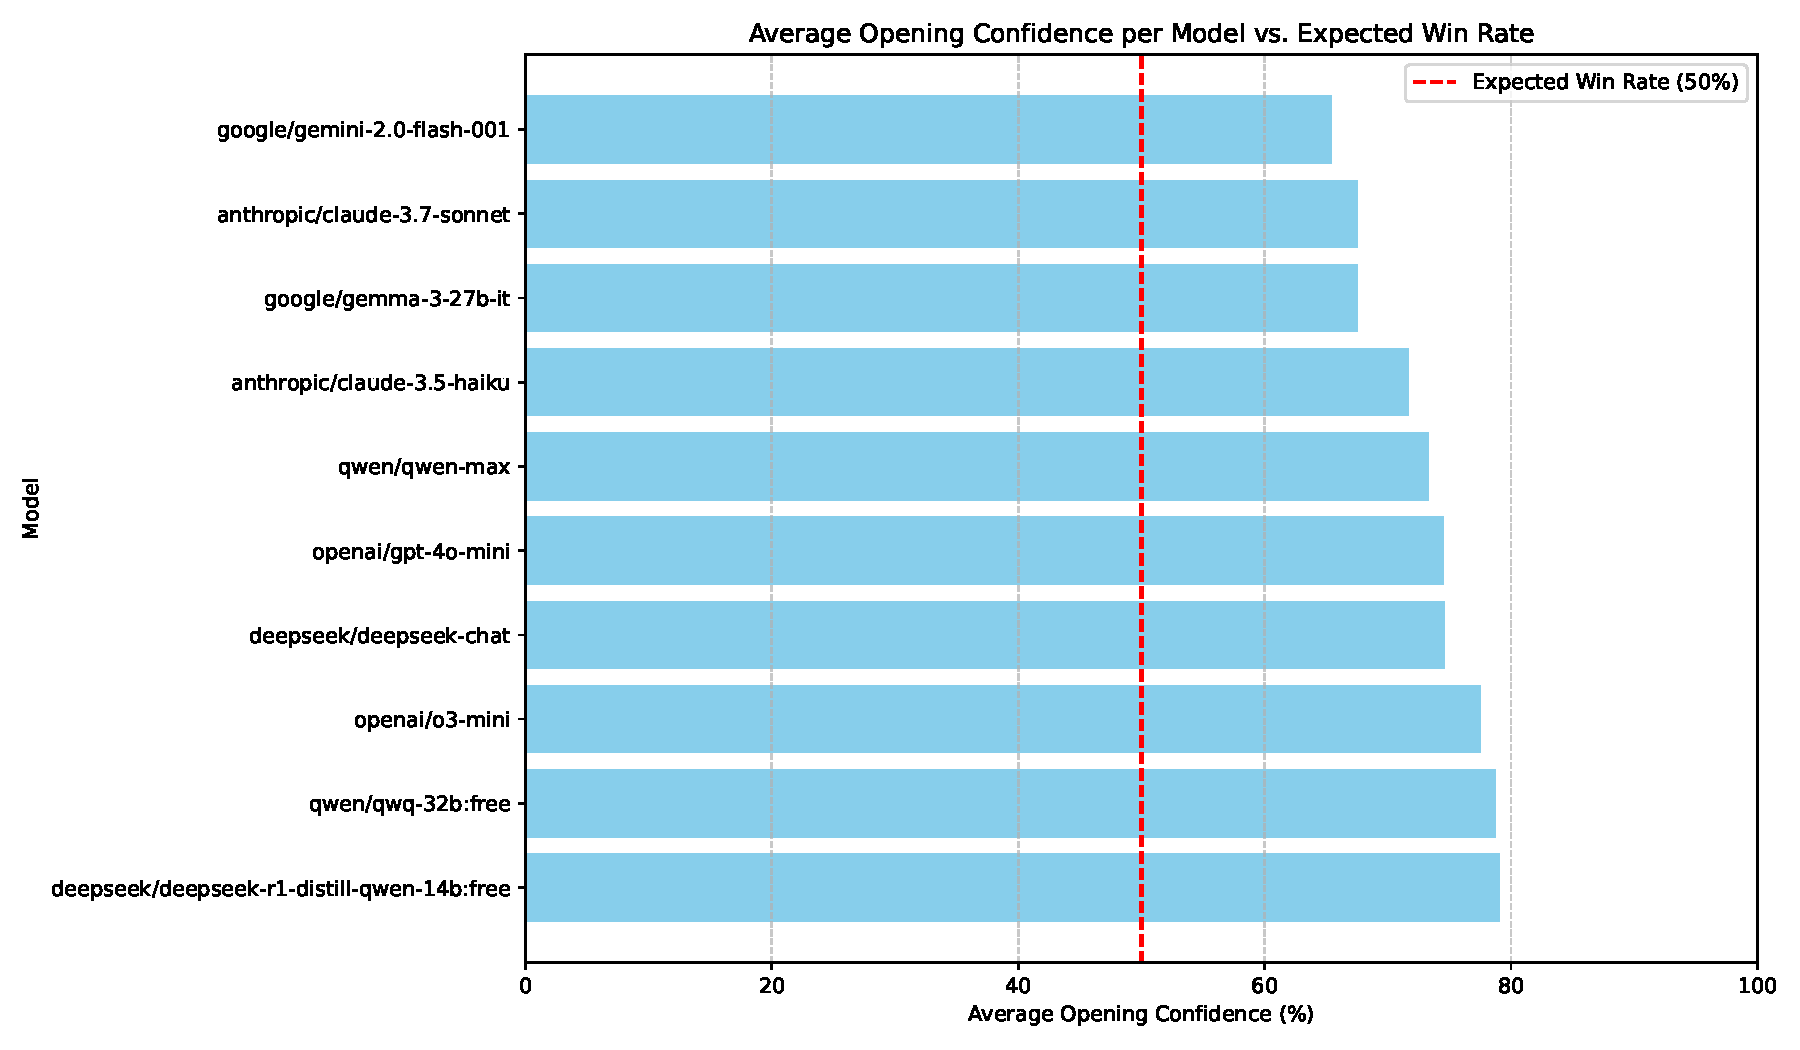
\includegraphics[width=0.8\linewidth]{figures/model_avg_opening_confidence_bar_chart.pdf}
  \caption{Average stated confidence in the first round across all LLMs and rounds compared to the expected 50\% win rate.}
  \label{fig:avg_confidence}
\end{figure}

\subsection{Position Asymmetry and Confidence Mismatch}

The AI jury evaluations revealed a significant advantage for the Opposition side in our debate setup. Opposition models won 71.2\% of the debates, while Proposition models won only 28.8\%. This asymmetry was highly statistically significant ($\chi^2(1, N=59) = 12.12, p < 0.0001$; Fisher's exact test $p < 0.0001$).

Despite this clear disparity in success rates, Proposition models reported \textit{higher} average confidence (74.58\%) than Opposition models (71.27\%) across all rounds. While the difference in confidence itself is modest, its direction is contrary to the observed outcomes and statistically significant (Independent t-test: $t(175) = 2.54, p = 0.0115$; Mann-Whitney U test: $U=4477, p = 0.0307$). This indicates that models failed to recognize or account for the systematic disadvantage faced by the Proposition side in this environment.

\begin{figure}[h]
  \centering
  % TODO: Replace with figure comparing Win Rate vs. Average Confidence for Proposition and Opposition sides
  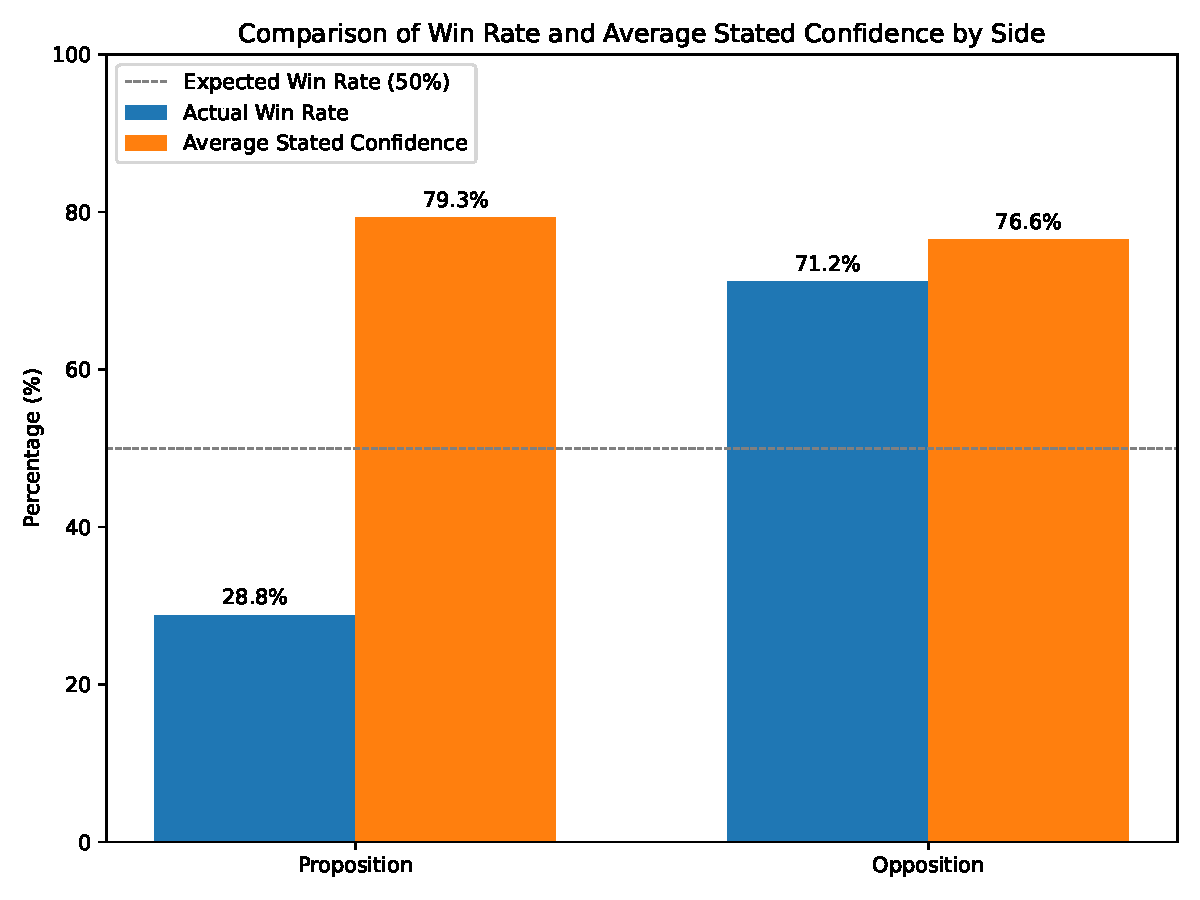
\includegraphics[width=0.8\linewidth]{figures/side_winrate_confidence_comparison.pdf}
  \caption{Comparison of Win Rate and Average Confidence for Proposition and Opposition sides.}
  \label{fig:position_bias}
\end{figure}

\subsection{Logically Impossible Confidence Scenarios}

A stark illustration of LLM metacognitive failure is the frequency with which both debaters expressed high confidence simultaneously. In 71.2\% of the 59 debates, both the Proposition and Opposition models rated their chance of winning at $\ge$ 75\% in at least one round. Given that only one side can win, this scenario is logically impossible under mutual exclusivity. This widespread occurrence highlights a profound inability for models to ground their confidence in the objective constraints of the task.


\subsection{Dynamic Confidence Revision and Escalation}

Contrary to the expectation that models would adjust their confidence downwards when presented with strong counterarguments or performing poorly, average confidence levels generally \textit{increased} over the course of the debate, regardless of the eventual outcome.

Table \ref{tab:confidence_escalation} summarizes the average confidence per round and the total change from Opening to Final round for each model.

\begin{table}[h]
  \caption{Average Confidence Bets by Round and Total Change per Model}
  \label{tab:confidence_escalation}
  \centering
  \begin{tabular}{lrrrr}
    \toprule
    Model                              & Opening (\%) & Rebuttal (\%) & Final (\%) & Change (Final - Opening) (\%) \\
    \midrule
    anthropic/claude-3.5-haiku         & 71.67   & 73.75    & 83.33   & +11.66 \\
    anthropic/claude-3.7-sonnet        & 67.50   & 73.75    & 82.92   & +15.42 \\
    deepseek/deepseek-chat             & 74.58   & 77.92    & 80.00   & +5.42  \\
    deepseek/deepseek-r1-distill-qwen-14b & 79.09   & 80.45    & 86.36   & +7.27  \\
    google/gemini-2.0-flash-001        & 65.42   & 63.75    & 64.00   & -1.42  \\
    google/gemma-3-27b-it              & 67.50   & 78.33    & 88.33   & +20.83 \\
    openai/gpt-4o-mini                 & 74.55   & 77.73    & 81.36   & +6.81  \\
    openai/o3-mini                     & 77.50   & 81.25    & 84.50   & +7.00  \\
    qwen/qwen-max                      & 73.33   & 81.92    & 88.75   & +15.42 \\
    qwen/qwq-32b:free                  & 78.75   & 87.67    & 92.83   & +14.08 \\
    \midrule
    Overall Average                    & 72.98   & 77.09    & 83.29   & +10.31 \\ % Calculated from table data
    \bottomrule
  \end{tabular}
\end{table}

Only one model (google/gemini-2.0-flash-001) showed a slight decrease in confidence (-1.42), while others increased their confidence significantly, with gains ranging up to +20.83 (google/gemma-3-27b-it). This "confidence escalation" occurred even for models that ultimately lost the debate, indicating a failure to incorporate disconfirming evidence or recognize the opponent's superior argumentation as the debate progressed.

\begin{figure}[h]
  \centering
  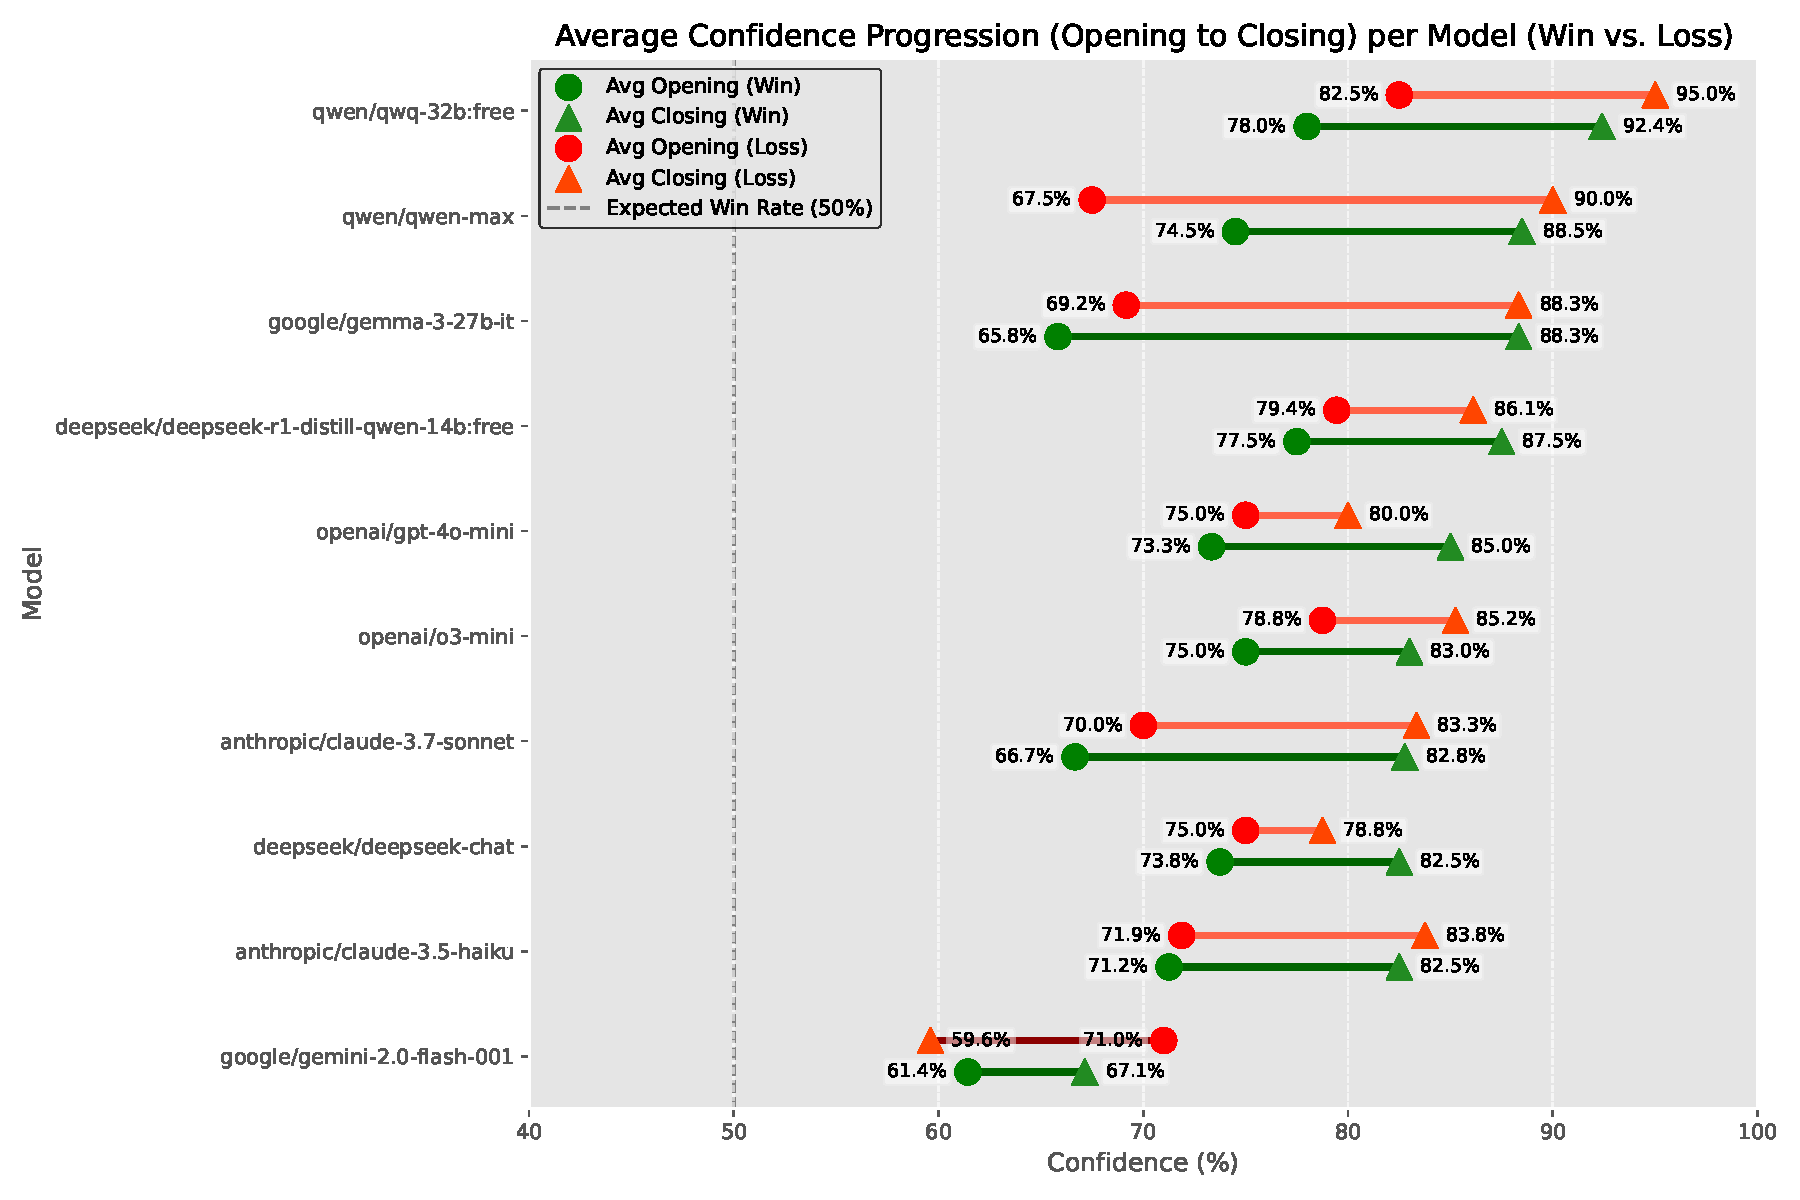
\includegraphics[width=0.9\linewidth]{figures/model_win_loss_escalation_dumbell.pdf}
  \caption{Confidence escalation across debate rounds for models that ultimately won versus models that ultimately lost.}
  \label{fig:confidence_trend_winner_loser}
\end{figure}

\subsection{Model-Specific Performance and Calibration}

Individual models varied in their overall performance (win rate) and calibration quality. We measured calibration using the Mean Squared Error (MSE) between the stated confidence (as a probability) and the binary outcome (win=1, loss=0), where lower MSE indicates better calibration. Calibration scores ranged from 0.1362 (qwen/qwen-max) to 0.5355 (deepseek/deepseek-r1-distill-qwen-14b:free), indicating substantial differences in the models' ability to align confidence with outcome.

\begin{table}[h]
  \caption{Model-Specific Debate Performance and Calibration Metrics}
  \label{tab:model_calibration}
  \centering
  \begin{tabular}{lcccc}
    \toprule
    Model                                   & Win Rate (\%) & Avg. Confidence (\%) & Overconfidence (\%) & Calibration Score (MSE) \\
    \midrule
    anthropic/claude-3.5-haiku              & 33.3          & 71.7                 & +38.4               & 0.2314 \\
    anthropic/claude-3.7-sonnet             & 75.0          & 67.5                 & -7.5                & 0.2217 \\
    deepseek/deepseek-chat                  & 33.3          & 74.6                 & +41.3               & 0.2370 \\
    deepseek/deepseek-r1-distill-qwen-14b   & 18.2          & 79.1                 & +60.9               & 0.5355 \\
    google/gemini-2.0-flash-001             & 50.0          & 65.4                 & +15.4               & 0.2223 \\
    google/gemma-3-27b-it                   & 58.3          & 67.5                 & +9.2                & 0.2280 \\
    openai/gpt-4o-mini                      & 27.3          & 74.5                 & +47.2               & 0.3755 \\
    openai/o3-mini                     & 33.3          & 77.5                 & +44.2               & 0.3826 \\
    qwen/qwen-max                           & 83.3          & 73.3                 & -10.0               & 0.1362 \\
    qwen/qwq-32b:free                       & 83.3          & 78.8                 & -4.5                & 0.1552 \\
    \bottomrule
  \end{tabular}
\end{table}

As shown in Table \ref{tab:model_calibration}, models varied widely in their overconfidence (Avg. Confidence - Win Rate). Some models like \texttt{qwen/qwen-max} and \texttt{qwen/qwq-32b:free} were slightly underconfident on average, achieving high win rates with relatively modest average confidence bets. Conversely, models like \texttt{deepseek/deepseek-r1-distill-qwen-14b:free}, \texttt{openai/gpt-4o-mini}, and \texttt{openai/o3-mini} exhibited substantial overconfidence.

Analyzing confidence tiers, models betting 76-100\% confidence won only 45.2\% of the time, slightly worse than those betting 51-75\% (51.2\% win rate). While there were limited data points for lower confidence tiers (only 1 instance in 26-50\% and 0 in 0-25\%), these findings suggest that high confidence in LLMs in this setting is not a reliable indicator of actual success.

Furthermore, a regression analysis using debate side (Proposition/Opposition) and average confidence as predictors of winning confirmed that while debate side was a highly significant predictor ($p < 0.0001$), average confidence was not ($p = 0.1435$). This reinforces that confidence in this multi-turn, adversarial setting was decoupled from factors driving actual debate success.

\subsection{Jury Agreement and Topic Characteristics}

The AI jury demonstrated moderate inter-rater reliability. 37.3\% of debate outcomes were unanimous (all 6 judges agreed), while 62.7\% involved split decisions among the judges. Dissenting opinions were distributed as follows: 1 dissenting judge (18.6\% of debates), 2 dissenting (32.2\%), and 3 dissenting (11.9\%). This level of agreement suggests the jury system provides a reliable, albeit not always perfectly consensual, ground truth for complex debate outcomes at scale.

Topic difficulty, as measured by the AI jury's difficulty index, varied across the six motions, ranging from the least difficult (media coverage requirements, 50.50) to the most difficult (social media shareholding, 88.44). This variation ensured that models debated across a range of complexity, although the core findings on overconfidence and calibration deficits were consistent across topics.



\section{Conclusion}
% Summarize your work and suggest future research directions.
% This is where you would place the content from the "Conclusion" section of your draft.

--- YOUR CONCLUSION CONTENT HERE ---

% --- Bibliography ---
% Use the environment below to include your bibliography.
% Make sure you have a file named "references.bib" in the same directory.
% You can use different bibliography styles (e.g., unsrtnat, abbrvnat),
% but plainnat is recommended by the template.

\bibliographystyle{plainnat} % Use plainnat or another natbib compatible style
\bibliography{references} % Your .bib file name (without extension)


% --- Acknowledgments ---
% Use the 'ack' environment for acknowledgments.
% This section is REQUIRED for the FINAL version of the paper but should be
% COMMENTED OUT or REMOVED for the ANONYMIZED SUBMISSION.
% The ack environment automatically hides this section in the default submission mode.
% For submission, ensure you declare funding and competing interests on the submission site,
% but *do not* include specific funding details in the paper body.
\begin{ack}
% Use unnumbered first level headings for the acknowledgments. All acknowledgments
% go at the end of the paper before the list of references. Moreover, you are required to declare
% funding (financial activities supporting the submitted work) and competing interests (related financial activities outside the submitted work).
% More information about this disclosure can be found at: \url{https://neurips.cc/Conferences/2025/PaperInformation/FundingDisclosure}.

% Do {\bf not} include this section in the anonymized submission, only in the final paper. You can use the \texttt{ack} environment provided in the style file to automatically hide this section in the anonymized submission.

% --- YOUR ACKNOWLEDGMENTS HERE (FOR FINAL VERSION ONLY) ---
This work was supported by [Funding Agency Name]. We thank [Names] for helpful discussions.
\end{ack}


% --- Appendix ---
% Optional section for technical appendices and supplementary material.
% This section and its content do NOT count towards the page limit.
% Ensure this comes AFTER the references in the camera-ready version if included in the same PDF.
% For submission, supplementary material can often be submitted as a separate file.
\appendix

\appendix

% Add these specific appendix sections here, after the \appendix command

\section{LLMs in the Debater Pool}
\label{appendix:llms}
This appendix lists the specific LLMs used in the debater pool for the experiments, including their names, providers, and potentially version information. [Content to be added]

\section{Debate Pairings Schedule}
\label{appendix:pairings}
This appendix details the schedule and method used for pairing LLMs against each other across different debate topics, ensuring a balanced experimental design. [Content to be added]

\section{Debater Prompt Structures}
\label{appendix:debater_prompts}
Full verbatim text of the structured prompts used to guide debater models in the Opening, Rebuttal, and Final rounds, including constraints and judging guidance. [Content to be added]

\section{AI Jury Prompt Details}
\label{appendix:judge_prompt}
Full verbatim text of the detailed prompt provided to the AI jury models for evaluating debate transcripts, including judging criteria and output requirements. [Content to be added]

\section{Topics of Debate}
\label{appendix:topics}

\section{Technical Appendices and Supplementary Material}
% Add detailed proofs, additional experimental results, larger figures, or other
% supplementary information here.
% This section does not count towards the page limit.

--- YOUR APPENDIX CONTENT HERE (OPTIONAL) ---

% Example: Detailed Proof
% \section{Proof of Theorem 1}
% --- Proof steps here ---

% Example: Additional Experimental Results
% \section{Additional Results}
% --- More tables or figures ---


% --- NeurIPS Paper Checklist ---
% REQUIRED for ALL submissions.
% This section does NOT count towards the page limit and should follow the appendix.
% Delete the instruction block within this section.
% Answer each question with \answerYes{}, \answerNo{}, or \answerNA{}
% Provide a brief justification for each answer.

\newpage % Optional: Start checklist on a new page

\section*{NeurIPS Paper Checklist}

%%% BEGIN INSTRUCTIONS %%%
% The checklist is designed to encourage best practices for responsible machine learning research...
% DELETE THIS INSTRUCTION BLOCK BEFORE SUBMISSION
%%% END INSTRUCTIONS %%%

\begin{enumerate}

\item {\bf Claims}
    \item[] Question: Do the main claims made in the abstract and introduction accurately reflect the paper's contributions and scope?
    \item[] Answer: \answerTODO{} % Replace by \answerYes{}, \answerNo{}, or \answerNA{}.
    \item[] Justification: \justificationTODO{} % Provide 1-2 sentence justification.

\item {\bf Limitations}
    \item[] Question: Does the paper discuss the limitations of the work performed by the authors?
    \item[] Answer: \answerTODO{} % Replace by \answerYes{}, \answerNo{}, or \answerNA{}.
    \item[] Justification: \justificationTODO{}

\item {\bf Theory assumptions and proofs}
    \item[] Question: For each theoretical result, does the paper provide the full set of assumptions and a complete (and correct) proof?
    \item[] Answer: \answerTODO{} % Replace by \answerYes{}, \answerNo{}, or \answerNA{}.
    \item[] Justification: \justificationTODO{}

    \item {\bf Experimental result reproducibility}
    \item[] Question: Does the paper fully disclose all the information needed to reproduce the main experimental results of the paper to the extent that it affects the main claims and/or conclusions of the paper (regardless of whether the code and data are provided or not)?
    \item[] Answer: \answerTODO{} % Replace by \answerYes{}, \answerNo{}, or \answerNA{}.
    \item[] Justification: \justificationTODO{}

\item {\bf Open access to data and code}
    \item[] Question: Does the paper provide open access to the data and code, with sufficient instructions to faithfully reproduce the main experimental results, as described in supplemental material?
    \item[] Answer: \answerTODO{} % Replace by \answerYes{}, \answerNo{}, or \answerNA{}.
    \item[] Justification: \justificationTODO{}

\item {\bf Experimental setting/details}
    \item[] Question: Does the paper specify all the training and test details (e.g., data splits, hyperparameters, how they were chosen, type of optimizer, etc.) necessary to understand the results?
    \item[] Answer: \answerTODO{} % Replace by \answerYes{}, \answerNo{}, or \answerNA{}.
    \item[] Justification: \justificationTODO{}

\item {\bf Experiment statistical significance}
    \item[] Question: Does the paper report error bars suitably and correctly defined or other appropriate information about the statistical significance of the experiments?
    \item[] Answer: \answerTODO{} % Replace by \answerYes{}, \answerNo{}, or \answerNA{}.
    \item[] Justification: \justificationTODO{}

\item {\bf Experiments compute resources}
    \item[] Question: For each experiment, does the paper provide sufficient information on the computer resources (type of compute workers, memory, time of execution) needed to reproduce the experiments?
    \item[] Answer: \answerTODO{} % Replace by \answerYes{}, \answerNo{}, or \answerNA{}.
    \item[] Justification: \justificationTODO{}

\item {\bf Code of ethics}
    \item[] Question: Does the research conducted in the paper conform, in every respect, with the NeurIPS Code of Ethics \url{https://neurips.cc/public/EthicsGuidelines}?
    \item[] Answer: \answerTODO{} % Replace by \answerYes{}, \answerNo{}, or \answerNA{}.
    \item[] Justification: \justificationTODO{}

\item {\bf Broader impacts}
    \item[] Question: Does the paper discuss both potential positive societal impacts and negative societal impacts of the work performed?
    \item[] Answer: \answerTODO{} % Replace by \answerYes{}, \answerNo{}, or \answerNA{}.
    \item[] Justification: \justificationTODO{}

\item {\bf Safeguards}
    \item[] Question: Does the paper describe safeguards that have been put in place for responsible release of data or models that have a high risk for misuse (e.g., pretrained language models, image generators, or scraped datasets)?
    \item[] Answer: \answerTODO{} % Replace by \answerYes{}, \answerNo{}, or \answerNA{}.
    \item[] Justification: \justificationTODO{}

\item {\bf Licenses for existing assets}
    \item[] Question: Are the creators or original owners of assets (e.g., code, data, models), used in the paper, properly credited and are the license and terms of use explicitly mentioned and properly respected?
    \item[] Answer: \answerTODO{} % Replace by \answerYes{}, \answerNo{}, or \answerNA{}.
    \item[] Justification: \justificationTODO{}

\item {\bf New assets}
    \item[] Question: Are new assets introduced in the paper well documented and is the documentation provided alongside the assets?
    \item[] Answer: \answerTODO{} % Replace by \answerYes{}, \answerNo{}, or \answerNA{}.
    \item[] Justification: \justificationTODO{}

\item {\bf Crowdsourcing and research with human subjects}
    \item[] Question: For crowdsourcing experiments and research with human subjects, does the paper include the full text of instructions given to participants and screenshots, if applicable, as well as details about compensation (if any)?
    \item[] Answer: \answerTODO{} % Replace by \answerYes{}, \answerNo{}, or \answerNA{}.
    \item[] Justification: \justificationTODO{}

\item {\bf Institutional review board (IRB) approvals or equivalent for research with human subjects}
    \item[] Question: Does the paper describe potential risks incurred by study participants, whether such risks were disclosed to the subjects, and whether Institutional Review Board (IRB) approvals (or an equivalent approval/review based on the requirements of your country or institution) were obtained?
    \item[] Answer: \answerTODO{} % Replace by \answerYes{}, \answerNo{}, or \answerNA{}.
    \item[] Justification: \justificationTODO{}

\item {\bf Declaration of LLM usage}
    \item[] Question: Does the paper describe the usage of LLMs if it is an important, original, or non-standard component of the core methods in this research? Note that if the LLM is used only for writing, editing, or formatting purposes and does not impact the core methodology, scientific rigorousness, or originality of the research, declaration is not required.
    %this research?
    \item[] Answer: \answerTODO{} % Replace by \answerYes{}, \answerNo{}, or \answerNA{}.
    \item[] Justification: \justificationTODO{}

\end{enumerate}


\end{document}
